\section{Statistical physics}\label{sec:stat_phys}
In formalising empirical observations of human gaze and neural activity into a mathematical model, this thesis relies on the framework of non-equilibrium statistical mechanics and stochastic calculus. When a system is driven by a massive number of microscopic interactions—such as the complex interconnected firing of a neural population—modelling the exact deterministic dynamics becomes intractable. Instead, statistical physics provides the tools to coarse-grain these high-dimensional systems into low-dimensional stochastic differential equations. This section establishes the mathematical progression necessary to model scale-free visual inference. We first review the classical paradigm of normal diffusion and Brownian motion (\cref{brown_mot}), which serves as the foundational null model for physical exploration. We then examine how biological systems frequently violate these classical assumptions, leading to anomalous diffusion (\cref{subsec:anom_diff}). Finally, we introduce Lévy stable motion (\cref{subsec:levy_motion}), a class of fractional stochastic processes that mathematically capture the heavy-tailed, intermittent dynamics characteristic of optimal visual search and neural activity.
\subsection{Brownian motion}\label{brown_mot}
Statistical modelling has been fundamental in understanding complex systems: separating the dynamics of macroscopic observables into deterministic terms and stochastic terms reduces high-dimensional systems to a small number of variables of interest \cite{hassler_stochastic_2016, cunchala2024basicoverviewvariousstochastic}. Across physics, economics, geology, climate science, machine learning, and neuroscience, stochastic processes are often the most natural, tractable, and accurate modelling choice when a system is too complex to model in full. The universality of these stochastic models is explained by the application of the central limit theorem, where the sum of very many small interactions over macroscopic time limits to a Gaussian random variable. This technique turns out to be generalisable to a wide class of coupled non-stationary processes out of equilibrium, as described in \textcite{Izvekov_2025_Mori}, whose techniques can describe the mean effect of a neuronal spiking patterns as demonstrated in \textcite{La_Camera_2022_meanfieldneuron}. Such processes thus produce the most ubiquitous stochastic process: the Wiener process $W_t$, equivalently called Brownian motion, which has stationary and independent Gaussian increments across all non-overlapping time intervals. The Wiener process is a very simple and analytically elegant model of the coarse-grained effect of very many small finite-variance interacting influences. A Wiener process is defined only by its timescale, with a variance over trajectories after time $t$ of $t$ itself. Wiener processes yield time series which are almost surely continuous but nowhere differentiable. The Wiener process is understood as a model of the long-time dynamics of a variable affected by very many small uncorrelated finite variance influences \cite{hassler_stochastic_2016}. Classical examples of processes modelled by the Wiener process are: the movement of a macroscopic particle in a non-turbulent fluid \cite{hassler_stochastic_2016}, the gravitational influence of an orbiting collection of stars on supermassive black holes \cite{Chandrasekhar1943, Merritt2007a}, and (arguably) the movement of low-volatility stock prices \cite{cunchala2024basicoverviewvariousstochastic}.

To include random variables such as Brownian motion in dynamical systems, physicists and mathematicians have developed the tools of stochastic calculus. Brownian motion about a potential landscape $V(\textbf{x})$ is often described in dynamical systems contexts in terms of the standard first order Langevin equation:
\begin{equation}\label{eq:langevin}
    d\textbf{x}_t = -\gamma \nabla V(\textbf{x}_t) dt + \sqrt{2 \gamma} dW_t 
\end{equation}
Where the constant $\gamma$ describes the noise strength of the Brownian motion. To describe how the probability distribution of this walker $p(\textbf{x},t)$ evolves through time, the Fokker-Planck equation is used. In the case of \cref{eq:langevin}, the Fokker-Planck equation is:
\begin{equation}\label{eq:overdamped-fokkerplanck}
    \partial_t p(\textbf{x},t) = \frac{\gamma}{2} \nabla \cdot \left( p(\textbf{x},t) \nabla V(\textbf{x}) + \nabla p(\textbf{x},t) \right)
\end{equation}
whose unique stationary distribution is the Boltzmann-Gibbs distribution with $k_B T = 1$:
\begin{equation}\label{eq:boltzmann-gibbs}
    \pi(\textbf{x}) \propto \exp[-V(\textbf{x})]
\end{equation}
which yields the important relationship, where a potential can be constructed from a normalised target density via $V(\textbf{x}) = -\log \pi(\textbf{x})$. Importantly, the dynamical system defined by \cref{eq:langevin} is ergodic, and thus under \cref{eq:overdamped-fokkerplanck}, any initial distribution will converge to $\pi(\textbf{x})$. The Fokker-Planck equation for the standard Brownian-Langevin system is a diffusion PDE equivalent to the heat equation with a gradient term, a correspondence well-understood before the development of stochastic calculus. The diffusion arising from such small uncorrelated perturbations of a dynamical system leads to the statistical properties which first drove the study of statistical physics, such as normal diffusion and the universality of Brownian motion, which we follow in \cref{subsec:anom_diff} and \cref{subsec:levy_motion} respectively, however the neural system described in this thesis diverges strongly from the Brownian paradigm, requiring an understanding of fractional processes.

\subsubsection{Further stochastic models}
Only recently have the universality of stochastic processes asides from the Wiener process been well-studied. Of interest to this thesis is the case where microscopic perturbations become correlated and yield heavy-tailed statistics. Correlated steps, long-time memory effects, and chaotic microscopic dynamics can result in a stochastic process which does not limit to a Brownian motion \cite{Brevitt2025, Klages2013}. Of interest to us is the fractional \textit{Lévy flight}, a process driven by scale-free noise which span across many orders of magnitude. For instance, a spiking neural network at with diverging activity correlation length, where the centre of mass of neural firing is then subject to large jump discontinuities \cite{La_Camera_2022_meanfieldneuron, qi_fractional_2022, qi_fractional_2022}. Such large jumps in time series' are modelled with to Lévy stable noise, where the increments are drawn independently from a heavy-tailed distribution. This section describes the analytics, stability, and behaviour of such Lévy processes for our current study, and how their diffusive properties differ from the behaviour of Brownian motion.

\subsection{Anomalous diffusion}\label{subsec:anom_diff}
A key motivation for the development of such stochastic modelling of phenomena in nature was the study of diffusion. The universality of \textit{normal diffusion} in systems which are driven by Brownian motion has been studied closely, such as in the movement of particles in a fluid \cite{klafter_anomalous_2005, metzler_anomalous_2014, Merritt2007a}. It had been discovered prior to the development of the Fokker-Planck formalism that the free isotropic motion of such Brownian trajectories follow an evolving probability distribution $P(\textbf{x},t)$, whose dynamics are given by
\begin{equation}
    \partial_t P(\textbf{x},t) = D \nabla_{\textbf{x}}^2 P(\textbf{x},t)
\end{equation}
where $D$ is some scaling constant. The solution to this is simple, as this is the heat equation. Thus, this can be solved as $P(\textbf{x},t) \propto \exp\left[ -\frac{\|\textbf{x} \|^2}{2(2Dt)}\right]$, showing that the variance of this distribution will scale as $2Dt$. These dynamics inform the definition of \textit{normal diffusion} through this variance scaling with time, rigorously calculated as the mean squared displacement (MSD) $\langle \|\Delta x (t) \|^2 \rangle = 2Dt$. This MSD linear in time defines normal diffusion. Such normal diffusion is universal to any realisation of Brownian motion, and thus any finite-variance aggregated process. To study such diffusive random walks and their long time behaviour, German physicist Albert Einstein and the British statistician Karl Pearson independently developed the continuous time random walk (CTRW) model, in which a trajectory has subsequent step sizes and durations drawn from finite variance distributions. Such models will universally reproduce this normal diffusive scaling property of $\langle \| \Delta x (t) \| \rangle \propto t$, and as a result of the central limit theorem, will approach Brownian motion. However, increasingly interesting physical systems have been found which diffuse nonlinearly in time, a situation known as anomalous diffusion, with an MSD scaling as:
\begin{equation}
    \langle \| \Delta x (t) \| \rangle \propto t^{\beta}, \ \ \beta \neq 1
\end{equation}
Such anomalous diffusion yields two cases, subdiffusion $0 < \beta < 1$ where diffusion scales slower than normal, and superdiffusion $1 < \beta < 2$ where diffusion scales faster than normal. The case of $\beta = 2$ is known as ballistic diffusion, as it is found in the deterministic case of constant velocity $x = vt$. Anomalous subdiffusion has been shown to result from heavy-tailed wait-times between interactions \cite{klafter_anomalous_2005}, such as in trapped fluid flow \cite{Kirchner2000-kf}, controlled diffusion through cell membranes \cite{klafter_anomalous_2005}, and protein mixing \cite{Kou2004-kz}. Later in \cref{subsec:levy_motion}, we will find that it is advantageous in the study of superdiffusive anomalous diffusion to extend the MSD to further fractional absolute displacements (FAD), which consider other scaling patterns of $\| \Delta x(t)\|$.
\subsubsection*{Anomalous superdiffusion}\label{subsubsec:anomalous_superdiffusion}
More importantly to this thesis, superdiffusion has been studied in the contexts of complex exploratory biological systems. Superdiffusion has a strong link to the problem of a blind search for scarce resources, however the true computational benefit of superdiffusion has become a subject of debate in the literature. On one side, the Lévy foraging hypothesis posits that the standard superdiffusive CTRW, the Lévy walk, is an optimal strategy when searching for sparse and randomly distributed resources. This result was first reported in a letter to the journal Nature in 1999 by \textcite{viswanathan_optimizing_1999}. However, recent physicists and biologists have questioned if this is instead an artefact of improper modelling, an argument led by described most strongly this year by \textcite{pyke_levy_2026}. In the original paper proposing the Lévy foraging hypothesis a Lévy walk with superdiffusion $\langle x(t) ^2 \rangle \propto \frac{t^2}{\ln(t)}$ on the transition to ballistic diffusion was found to be optimal in a search for sparse resources \cite{viswanathan_optimizing_1999}. Further, the optimality of the superdiffusive Lévy walk has been reproduced in diverse functional search models \cite{humphries_optimal_2014, campeau_evolutionary_2022, sims_optimal_2019}, in a population of diverse searching agents with a range of superdiffusive exponents \cite{clementi_search_2021}, and have been reported in the empirical search paths of biological organisms from the flights of drosophila flies \cite{sims_optimal_2019, reynolds_free-flight_2007}, albatross' searches \cite{focardi_levy_2014, humphries_new_2013}, and strongly across many marine predators \cite{sims_scaling_2008, humphries_environmental_2010}. Despite these analyses, advantages of Lévy walks have been shown to be model-dependent, with the optimal performance of Lévy walks requiring biologically inaccurate depictions of search paths \cite{pyke_levy_2026, gautestad_levy_2013, pyke_understanding_2015}. These arguments marks a split in the treatment of Lévy walks, with groups studying them as informative baseline functional models of abstract search \cite{viswanathan_optimizing_1999, gautestad_levy_2013, humphries_optimal_2014, clementi_search_2021}, and others led by Graham Pyke presenting this as a misrepresentation of true intelligent organisms \cite{pyke_levy_2026, pyke_understanding_2015, benhamou_ultimate_2015}. This thesis provides a biologically realistic and well-motivated superdiffusive search for research into a case for optimal Lévy motion. See \textcite{reynolds_liberating_2015} for an in-depth discussion of a richer view of biological Lévy walk superdiffusion.
% Simulating trajectories from stochastic processes such as Wiener processes and Lévy flights are computationally direct, it is often useful to understand the dynamics of the distribution of trajectories after some time $t$. The dynamics of the distribution of trajectories driven by a stochastic differential equation is defined through the Fokker-Planck Equation (FPE), also known as the Kolmogorov Forward Equation. The paradigmatic FPE is given for the Langevin Equation:
% \begin{equation}
% 	dX_t = \mu(X_t,t)dt + \sigma(X_t,t) dW_t
% \end{equation}
% giving the partial differential equation for the distribution $p(x,t)$ of $X_t$:
% \begin{equation}
% 	\frac{\partial p(x,t)}{\partial t} = - \frac{\partial}{\partial x} [ \mu(x, t)p(x,t) ] + \frac{1}{2} \frac{\partial^2}{\partial x^2}[\sigma^2(x,t)p(x,t)]
% \end{equation}
% In the case where $\mu(x,t) = 0$ and $\sigma(x,t) = \sigma$, the Langevin FPE simplifies into the standard heat equation, with diffusion of the probability mass with a rate defined by the volatility parameter $\sigma$:
% \begin{equation}
% 	\frac{\partial p(x,t)}{\partial t} = \frac{\sigma^2}{2} \nabla^2 p(x,t)
% \end{equation}
% The heat equation is very well studied, and given an initial condition concentrated at the point $(x,t) = (x_0,0)$, the distribution at any time $t>0$ is exactly a Gaussian defined by:

% \begin{equation}
% 	p(x,t) = \frac{1}{(2 \pi \sigma^2 t)^{1/2}} \exp \left( - \frac{|x|^2}{2 \sigma^2 t} \right)
% \end{equation}

% We see from this that the variance of such a distribution will scale as $\textbf{Var}_x[p(x,t)] \propto t$

\subsection{Lévy stable motion}\label{subsec:levy_motion}
To mathematically capture the intermittent, scale-free nature of visual search, we turn to the \textit{Lévy flight}: a superdiffusive stochastic process that permits close analysis, due to it's very foundational mathematical definition. Here, the Lévy flight $L_t^{\alpha}$ is a stochastic process defined through it's increments being drawn from a heavy tailed symmetric $\alpha$-stable distribution (a $\mathcal{S}\alpha\mathcal{S}$ distribution), where $\alpha$ is called the characteristic exponent and relates to the exponent of the distributions powerlaw tails. $\mathcal{S}\alpha\mathcal{S}$ distributions describe the limit of summation of i.i.d infinite-variance variables, as a result of the generalised central limit theorem, making them ideal to describe a universality class of superdiffusive processes. The $\alpha$ value defining a particular $\mathcal{S}\alpha\mathcal{S}$ distribution is a result of the asymptotic power-law tail of the density function, with the probability density function following $p(x) \propto |x|^{-1-\alpha}$. As a result, the Lévy flight $L_t^{\alpha}$ after time $t$ is defined by its fractional scaling properties and alpha-stable statistics
\begin{equation} \label{eq:levy_noise}
	L_t \stackrel{d}{=} t^{1/\alpha} L_1, \ \ L_1 \sim \mathcal{S}\alpha\mathcal{S}
\end{equation}
where $\stackrel{d}{=}$ denotes equal in distribution. In the limit $\alpha \rightarrow 2$, the Lévy flight reduces to a scaled Brownian Motion $L_t^{\alpha \rightarrow 2} = \frac{1}{\sqrt{2}}W_t$. If $1 < \alpha < 2$ the variance of $L_t^{\alpha}$ diverges and has mean 0, whereas if $0 < \alpha \leq 1$, then both the variance and mean diverge. In analysing the distribution of a Lévy flight, one must generalise the standard Langevin Fokker-Planck equation (\ref{eq:overdamped-fokkerplanck}) to the Lévy motion using fractional calculus to capture the nonlocal transport of the particle. The details of such an analysis are beyond this thesis, however the fractional Fokker-Planck equation is the tool used to understand the superdiffusion, nonlocality, and scale-free behaviour of trajectories of Lévy flights (see the appendices to \cite{qi_fractional_2022}). Many of the simple analytic properties of the Wiener process are no longer true of a Lévy flight. Notably, since these flights have infinite variance in steps sizes, the mean squared displacement diverges. Thus their superdiffusion is better measured using an extension of MSD to fractional absolute displacements, through the definition of the moment spectrum function $\lambda(q)$ as in \cite{vilk_strong_2025}:
\begin{equation}\label{eq:MFD}
	\langle \| \Delta x(t) \| ^ q \rangle \propto t^{\lambda(q)}, \ \ q > 0
\end{equation}
where $q$ is the order of the fractional absolute displacement, and the power law slope will converge for an $\alpha$-Lévy flight to $\lambda(q) = q/\alpha$ when $q < \alpha$. As such, for Lévy flights with exponents $\alpha > 1$ superdiffusion is well-characterised by the mean absolute displacement, where $q=1$ in \cref{eq:MFD}.
\\ \hfill \break
\begin{figure}[h!]
	\centering
	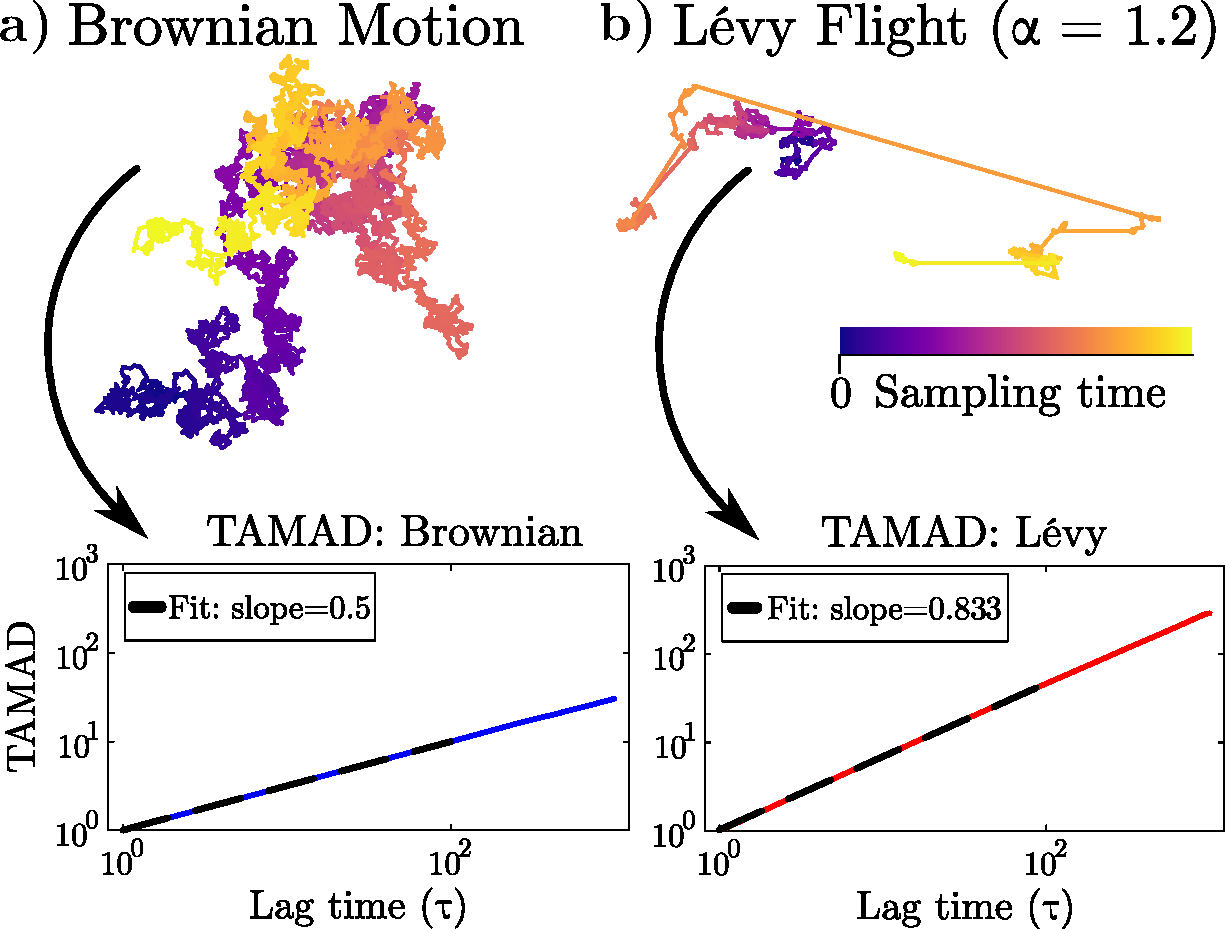
\includegraphics[width=0.8\linewidth]{figures/BvL.pdf}
	\caption{\textbf{Schematic representations of stochastic motion and their respective diffusion.} \textbf{a)} Schematic representation of a 2D Brownian motion, along with its time-averaged mean absolute displacement (TAMAD), which is the $q=1$ mean fractional displacement as in \cref{eq:MFD}. Normal diffusion is here present as a power law slope of exponent $1/2$, giving diffusive exponent $\beta=1$ as defined in \cref{eq:MFD}. \textbf{b)} Schematic of a superdiffusive 2D Lévy flight with characteristic exponent of $\alpha=1.2$, and a MAD slope of $0.833$ corresponding to the theoretical superdiffusive coefficient $\beta= 2/\alpha = 5/3$.}
	\label{fig:brownian_vs_levy}
\end{figure}
\\ \hfill \break
Importantly, trajectories of a Lévy flight are no longer continuous. Instead, such trajectories are called \textit{càdlàg} (continue à droite, limite à gauche) with respect to time, which describes functions which are right continuous with well-defined left limits \cite{van_den_Bosch}. Thus, we say that since all such trajectories produced from a Lévy flight are càdlàg, the Lévy flight itself is called a càdlàg process. Càdlàg processes have been widely studied in the context of mathematics, economics, and physics, and their properties are well understood \cite{soulier2022-ge, Borkar1995}. It has been shown that Lévy flights are semimartingales, and are well interpreted in integration \cite{van_den_Bosch}. Importantly, it follows from the Lévy-Itô decomposition theorem that a Lévy flight can be decomposed as the sum of two processes \cite{Kyprianou2014}:
\begin{enumerate}
	\item A compound Poisson process of large jumps with $|\Delta x| > 1$. Such jumps are exponentially distributed in time, and there are almost surely a finite number of such jumps in any finite time period.
	\item A square-integrable martingale (mean 0) jump process with $|\Delta x| < 1$. This process is then finite-variance, and as such is subject to the central limit theorem, meaning that under temporal coarse graining it approaches a Wiener process.
\end{enumerate}
This division is useful in analysing the process in the context of nonlocal stochastic exploration in Lévy flights, which is modelled by the compound Poisson process of large jumps $|\Delta x| > 1$, and the local exploitation dynamics modelled by the square-integrable martingale of small jumps $|\Delta x| < 1$. In the context of visual searching, such a division naturally inspires the division between large jumps of attention, and periods of prolonged attention. As such, we are interested in why such superdiffusive scale-free dynamics may have a powerful in computational advantage in exploring an abstract unknown landscape.

\subsection{Nested oscillations}